\documentclass{beamer}
\usepackage{mathtools, amsmath, xcolor, graphicx}
\usetheme{Rochester}
\usecolortheme{dolphin}

\author{Joe Bentley and Jake Lane}

\title{Higgs Signal Optimisation}

\institute{}
\subject{Physics}
\date{}
\begin{document}

\frame{\titlepage}

\frame{
\frametitle{Decay mechanism}
\begin{figure}
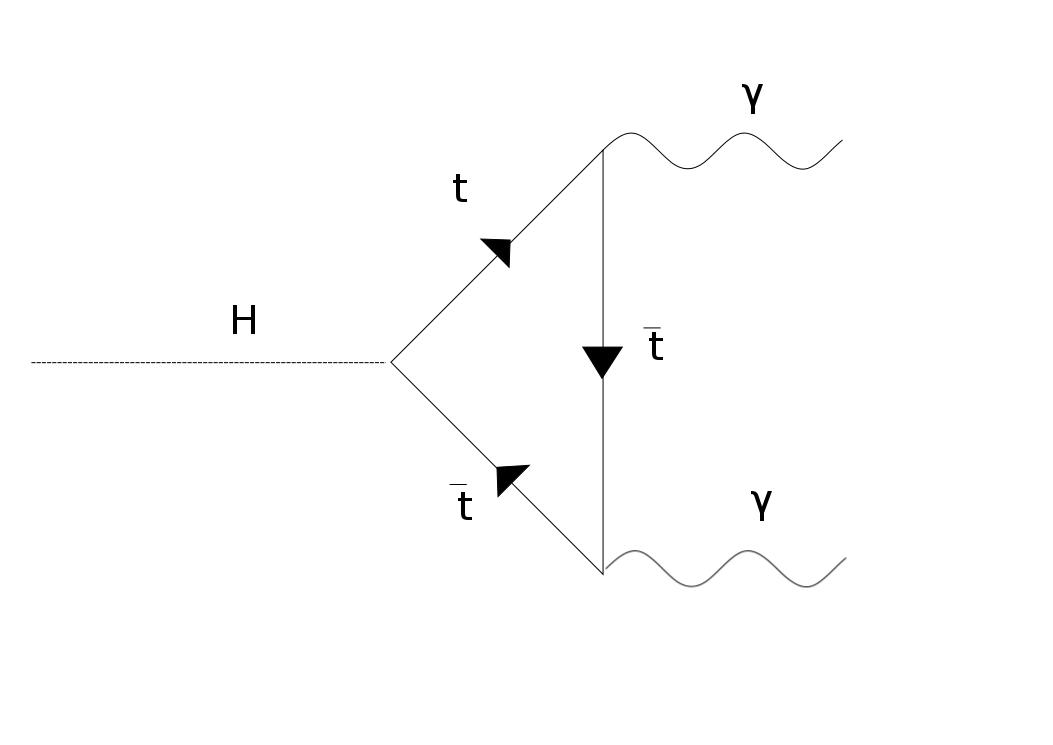
\includegraphics[scale = 0.25]{Hyy}
\caption{Higgs decay, $H$, into 2 photons, $\gamma$, via a top, $t$, quark loop}
\end{figure}
}

\frame{
\frametitle{Branching fraction}
\begin{enumerate}
\item Ratio of Higgs decays to photons over ratio of all Higgs decays.
\item Branching fraction $B$ for Higgs to 2 photons is of order $10^{-3}$.
\end{enumerate}
}

\frame{
\frametitle{Cross section}
\begin{enumerate}
\item Probability of producing a Higgs in an interaction, $\sigma_H$.
\item Summed over all possible production modes (most common is the gluon gluon fusion)
\end{enumerate}
\begin{equation}
\sigma_H = \sigma
\end{equation}
}

\frame{
\frametitle{Weighting}

Probability of producing a Higgs and decaying into 2 photons, compared to the probability of producing 2 background photons, $P$.
\begin{equation}
P = \frac{\sigma_H B_{\gamma \gamma}}{\sigma_{b}}
\end{equation}
}

\frame{
\frametitle{Kinematic variables}
Define 4-momentum by the following parameters:
\begin{align}
E = p^t &= p_T \cosh{\eta} \\
p^x &= p_T \cos{\theta}\\
p^y &= p_T \sin{\theta}\\
p^z &= p_T \sinh{\eta}
\end{align}
}
\frame{
\frametitle{Principle behind selection cuts}
\begin{enumerate}
\item Higgs decaying into 2 photons will have a distinct signature compared to simulated background.
\item This signature manifests in 2 high energy photons back to back.
\item Further expect the diphoton system to have an invariant mass in the range of measured mass of Higgs.
\end{enumerate}
}
\frame{
\frametitle{Energy cuts}
\begin{enumerate}
\item Photons produced in a Higgs decay have a large energy.
\item Photons do not get equal distribution of energy from a Higgs decay.
\end{enumerate}
}

\frame{
\frametitle{Transverse cut}
\begin{enumerate}
\item Magnitude of the momentum perpendicular to the beam, $p_T = \sqrt{p_x^2 +  p_y^2}$
\item Photons will get most of their energy from the Higgs decaying outwards from the beam.
\item Similar to the energy filter in construction.
\end{enumerate}
}

\frame{
\frametitle{Cuts using angular distance}
\begin{enumerate}
\item Ideally the Higgs produces photons back to back
\item Take both the square difference in rapidity, $\eta$ and square difference in azimuthal angle $\phi$.
\end{enumerate}
}

\frame{
\frametitle{Challenges to project}
}
\end{document}
